\documentclass[a4paper]{ctexart}

\usepackage{fontspec, xunicode}
\usepackage{amsmath}
\usepackage{amssymb}
\usepackage{latexsym}
\usepackage{graphicx}
\graphicspath{{./img/}}
\DeclareGraphicsExtensions{.png,.pdf}
\usepackage{subfig}
\usepackage{mathrsfs}
\usepackage{xeCJK}
\usepackage[dvipsnames, svgnames, x11names]{xcolor}
\usepackage{todonotes}
\usepackage{hyperref}
\usepackage{minted}

\usepackage{geometry}
\geometry{a4paper,left=2cm,right=2cm,top=3cm,bottom=3cm}


\begin{document}

\begin{titlepage}
    \centering
    \title{媒体与认知图像处理大作业\\实验报告}
    \vspace{\stretch{4}}
    \maketitle
    \author{张艺璇\quad 无64\quad 2016011081\\江振宇\quad 无67\quad 2016011165}
    \\
\end{titlepage}

\section{摘要}
本次实验中,我们实现了一套系统的代码框架,并在这个框架下复现了包括 DenseNet, ResNet, ML\_GCN~\cite{ML_GCN_CVPR_2019}, Class Activation Map(CAM)~\cite{zhou2016learning} 在内的多种算法,进行了多次实验。最终,我们采用 ML\_GCN 网络来实现多标签物体分类,利用 Hide and Seek 算法改进下的 CAM 实现了弱监督的物体检测。代码详见 \url{https://github.com/zyx16/Object-Classification} 或 code 文件夹中。


\section{引言}
多标签分类任务是计算机视觉领域中非常基础而且重要的任务之一。其应用包括但不限于医学诊断,人物特征识别。相比于单标签多分类任务,多标签分类任务更具有挑战性。因为多标签分类任务输出空间远比单标签复杂。

应用于多标签分类任务的网络模型大部分是基于传统 CNN 模型改进的结果,包括 VGG, ResNet, DenseNet 等。我们采用了效果比较好的 ResNet101 和 DenseNet161 并在其基础上进行改进。ResNet~\cite{he2016deep}的特点在于引入了 shortcut connection ,保护了原始图像中的信息不被破坏。 DenseNet~\cite{huang2017densely} 则将shortcut connection 进一步改进为 dense connection ,取得了更好的图像分类效果。

我们实现了基于 ResNet101 和 DenseNet161 的 ML-GCN~\cite{ML_GCN_CVPR_2019} 算法。这种算法利用了标签对应词语的词向量,和这些标签在训练集中出现的次数以及共同出现的次数,来挖掘标签之间的内部关系。不同的标签在图片中出现的概率是有关联的, ML-GCN 希望通过挖掘它们之间的内在关联来提高多标签分类的准确性。 ML-GCN 中, GCN 模块需要的输入是标签对应的词向量,在ML-GCN网络中除了权重矩阵和非线性激活单元之外,还需要预先统计并处理过的各个标签在图片中两两共同出现的次数,用这个网络来处理这些词向量,然后用 GCN 模块的输出结合 CNN 网络的输出,帮助改进多标签分类的结果。由于 GCN 模块和 CNN 网络的计算是完全独立进行的,只需要把它们的输出结果一起处理得到最终输出,所以 ML-GCN 具有很好的可移植性,可以添加到大部分分类网络上。我们的实验证明, ML-GCN 对衡量分类准确性的几种指标的确都有明显的改进效果。

弱监督的算法在诸多计算机视觉任务都有应用,如物体的分割,物体检测等等。弱监督物体检测(WSOD)很大的一个优点就在于它相比于一般的物体检测,需要的标注数据非常少。一般物体检测需要 bounding box 和 label 的 ground truth ,而弱监督的物体检测一般只需要图片级别的 label 作为 ground truth 。根据我们的调研,弱监督的物体检测主要有两大类方法:基于 region proposal 的方法和基于 discriminative area 的方法。前者一般是利用一些弱监督或无监督的 region proposal 方法得到候选的 bounding box ,再通过计算这些候选框的置信度来进行筛选。而后者则是通过卷积操作本身的空间相对不变性——一张特征图上一个点在图中的相对位置与其对应的感受野在原图中的相对位置一致——以及特征图上的值反应激活强度这两个特性,通过计算激活图来获得图中物体的相对位置的。基于 region proposal 的方法一般复杂度较高,但是检测准确率比较好;而基于 discriminative area 的方法一般复杂度较低,但是由于激活区域的种种限制,导致检测准确率较低,尤其在多目标的情况下。

我们采用了第二类方法,首先实现了 CAM~\cite{zhou2016learning} 方法,CAM 方法通过对 feature map 进行线性组合得到了 feature 的激活值,resize 到输入大小后,就可以得到对应原图的激活图。

我们又实现了基于 CAM 的 SoftProposal~\cite{zhu2017soft} 方法和 Hide and Seek~\cite{singh2017hide} 算法。SoftProposal 将特征图是为全连接的图,在图上进行特征的传播,将传播的结果作为特征图的权重因子以得到新的特征图。但是加入 SoftProposal 模块之后,由于其算法的复杂度,训练速度严重降低。通过用向量化操作替代循环,我们大大提高了运行速度,但是检测的准确率相比原始的 CAM 却有所下降,因此后面不再赘述此方法。

\begin{figure}[t]
   \centering
   \subfloat[激活图只关注人脸]{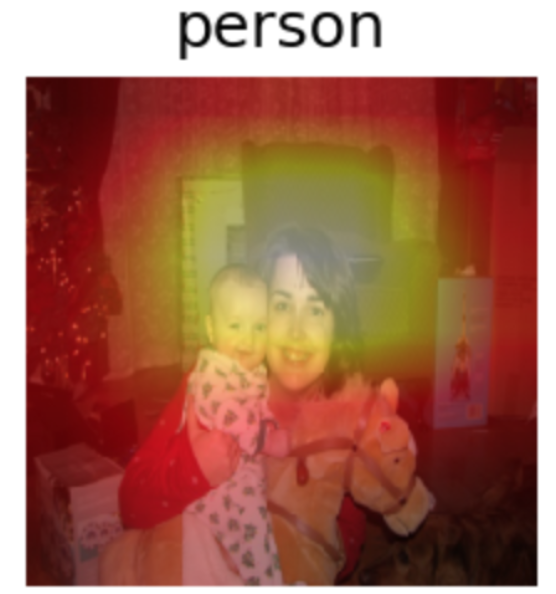
\includegraphics[width=0.4\textwidth]{person}%
   \label{fig:person}}
   \hfil
   \subfloat[通过掩盖图片的一部分,强制网络关注整体]{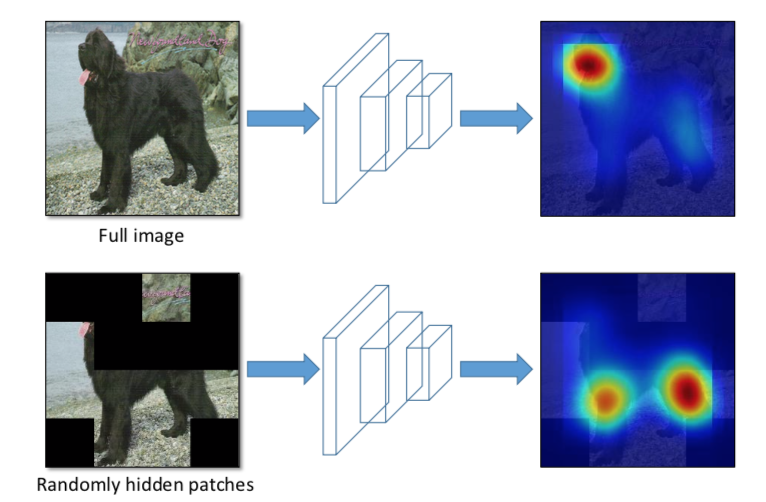
\includegraphics[width=0.55\textwidth]{dog}%
   \label{fig:dog}}
   \caption{CAM and Hide-and-Seek}
   \label{fig:CAM}
\end{figure}

Hide and Seek 算法则是一种简单巧妙而有效的算法。Hide and Seek 算法的提出基于这样一个观察,CAM 的激活图总是关注最显著的区域,比如图 \ref{fig:person} ,这是训练过程决定的,因为网络只需要关注到最显著的区域就可以判断某一类物体的存在与否。但是检测的目标是整个人体,因此检测的 IoU 会严重降低。\cite{singh2017hide} 提出,通过随机地掩盖图片中的一些块,就可以强制训练网络关注到那些不那么显著的区域,从而提升检测的准确率,如图 \ref{fig:dog}。

在使用 Hide and Seek 算法后,我们的检测 mAP 从 11.36\% 提高到了 12.07 \% 。

\section{文献综述}
\subsection{多标签分类}
常用的CNN分类模型包括AlexNet~\cite{krizhevsky2012imagenet}, VGG~\cite{simonyan2014very}, ResNet~\cite{he2016deep}, DenseNet~\cite{huang2017densely}等,实验中采用的主要是ResNet和DenseNet作为基础模型,在它们的基础上加以改进。

这些CNN模型用于分类的原理是提取出同类图像中相同的特征,其中ResNet的主要思想是在网络中加入了基于shortcut connection的identity mapping,表现为

    \begin{equation}
        x_l = H_l(x_{l-1}) + x_{l-1}
    \end{equation}

shortcut connection保护了原始图像中的信息,一定程度上解决了网络层数过深时梯度消失的问题。一个building block的示意见图\ref{fig:bottleneck building block in resnet101}。

	\begin{figure}[t]
		\small
		\centering
		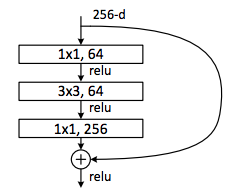
\includegraphics[width=4cm]{resnet.png}
		\caption{bottleneck building block in resnet101}
		\label{fig:bottleneck building block in resnet101}
	\end{figure}

DenseNet则通过层之间两两连接的dense connection进一步改进了网络结构。与ResNet不同的是,它的每一层的直接输入包含了前面所有层的信息,即

\begin{equation}
    x_l = H_l([x_{l-1}, x_{l-2},..., x_{0}])
\end{equation}

DenseNet主要由几个dense block和连接它们的transition layer组成。在dense block内部,每个layer是由 BN + Relu + Conv 构成的,这样的layer之间两两连接。如图\ref{fig:dense block}所示是一个五层组成的dense block示意图。

	\begin{figure}[t]
		\small
		\centering
		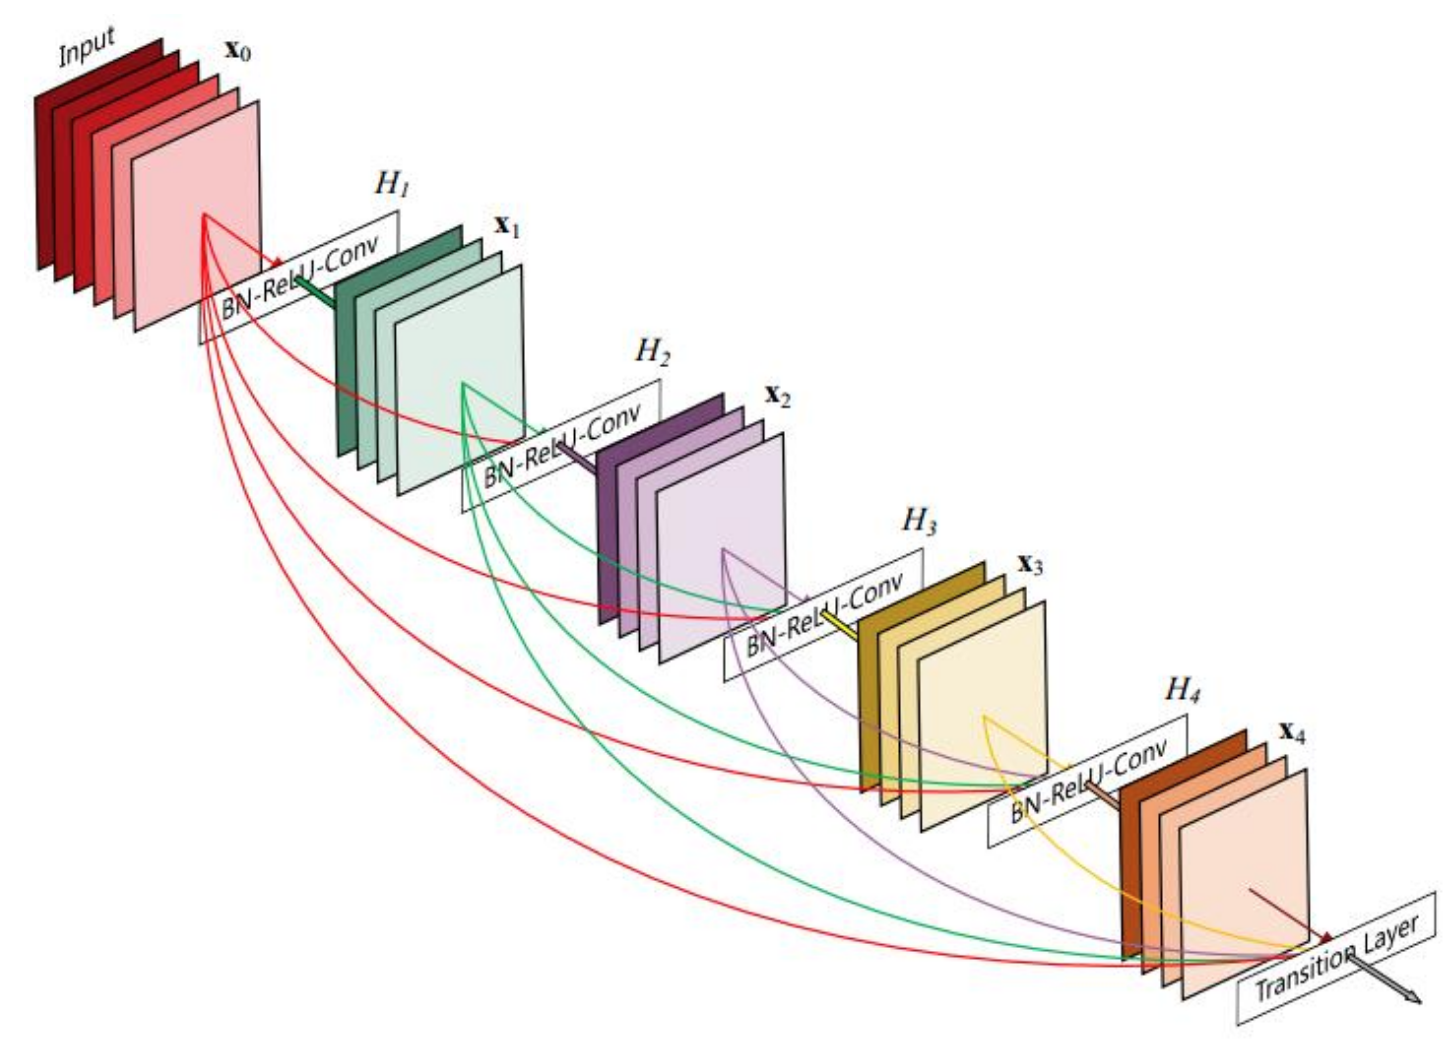
\includegraphics[width=7cm]{denseblock.png}
		\caption{a typical dense block}
		\label{fig:dense block}
	\end{figure}

在改进多标签分类效果方面, GCN 算法可以用于提取拓扑图的空间特征。通常的 CNN 在进行卷积操作时使用的是规则的卷积核,这也就导致 CNN 操作在图像处理以外的区域,比如一个普通意义上的由结点(node)和边(edge)组成的 graph 上比较难进行, GCN 是一种解决该问题的方式。

 GCN 应用于多标签分类,即 ML-GCN ~\cite{ML_GCN_CVPR_2019}时,将 ResNet 或其他CNN网络结构后的 classifier 替换成了 CNN 网络输出和 GCN 网络结构输出的乘积。 GCN 网络利用了词的向量表达,学习标签之间的内在联系,然后和 CNN 网络学习出的 feature 相乘。学习出的结果不需要再经过原本的线性 classifier ,而是直接作为预测的分类结果。



\subsection{WSOD}
全监督的卷积神经网络在物体检测上有着非常优秀的表现~\cite{ren2015faster, redmon2016you},但是需要很多精细的人工标注数据。而弱监督的物体检测需要的数据则少很多,比如在我们的实验中,我们只需要用到图片级别的 label 。正如引言中所说,解决这个问题的方法主要分为两大类:基于 region proposal 的方法和基于 discriminative area 的方法。前者一般利用一些弱监督或无监督的 region proposal 方法得到候选的 bounding box ,再进行进一步的筛选检测~\cite{bilen2016weakly, diba2017weakly, tang2018pcl}。Weakly Supervised Deep Detection Networks(WSDDN)~\cite{bilen2016weakly} 通过将预训练好的网络在卷积层后分为两支,分别实现分类和检测,分类是基于 Selective search~\cite{uijlings2013selective} 或者 EdgeBox~\cite{zitnick2014edge} 选出候选框后进行的。

基于 discriminative area 的方法则不需要 region proposal ,而是利用卷积的空间不变性和 feature map 的激活特性进行定位。其中比较著名的一篇就是~\cite{zhou2016learning}。这篇文章提出了 CAM:利用 Global Average Pooling(GAP),通过将最后的全连接矩阵对应某一类的参数作为权重,对最后一层 feature map 进行加权求和,合成的 feature map 就反映了激活强度。对激活图进行一些操作就可以得到 bounding box 。在 CAM 的基础上,又有一些文章提出了新的方法,对 CAM 做了一些改进~\cite{singh2017hide, zhu2017soft}。

\section{实验方案}
\subsection{数据预处理}

弱监督定位分类器的训练:resize 到 256*256 ,random crop 224*224 输入,用 imagenet 数据集的均值和方差来归一化。

\subsection{多标签分类}
\subsubsection{Baseline}
采用的baseline包括在多标签分类任务里表现优异的densenet和resnet。我们采用了 Pytorch 中 torchvision 库提供的在 imagenet 数据集上训练的 densenet161 和 resnet101 模型,将最后一层线性层的输出改为 20 类。

训练的细节如下:输出经过 Sigmoid ,得到每一类出现的概率。采用 BCEWithLogits 作为损失函数,训练时根据训练集每类出现的次数对每类的 loss 进行加权,出现次数多的 loss 的权重小,以达到平衡样本的目的。使用 ADAM 优化器,初始学习率是 $1\times10^{-4}$ ,在第 10 ,15 ,18 个 epoch 减半;weight decay 权重为 $1\times10^{-4}$。总训练代数为 20 。

\subsubsection{ML-GCN}

ML-GCN在baseline的基础上加入了GCN部分。用GLOVE训练好的300维词向量,提取出我们需要的20个标签对应的词向量送入GCN层。

ML-GCN 的模块包括两层 graph convolution 层。graph convolution 层的原理是
    \begin{equation}
        H^{l+1} = h(\hat{A}H^lW^l)
    \end{equation}
其中 $W^l$ 是参数,两层的 $\hat{A}$ 都是 adj 矩阵, 第一层的输入$H^l$是词向量矩阵;第二层的输入 $H^l$ 则是上一层的输出经过一层 relu 得到的结果。

其中 adj 矩阵的生成过程如下:首先统计 A 矩阵,它是训练集中的每两个不同标签共同出现次数的矩阵,对角元为0。然后分别将 A 矩阵的每行归一化并二值化。再将A和单位矩阵加权求和即得最终结果,单位矩阵代表每个标签的出现对自身的影响,可以防止标签间关系占比太重导致的 over-smoothing 。

二值化的阈值设为0.4,处理后的 A 和对角矩阵相加的比值为1:4,即 A 占比0.2,实际代码中是将A乘以0.25后和对角矩阵相加。

第一层输入的词向量矩阵和 label 本身有关。我们的数据集中一共有20个词,其中有的是短语,这种情况下我们采用的短语的第一个词。它们的词向量使用的是 GloVe ~\cite{Pennington14glove:global}算法在 wiki 数据集上训练过的300维词向量结果。



\subsection{WSOD}
% CNN
\subsubsection{分类器的训练}
在计算 CAM 之前,需要训练好一个分类器。在这里我们采用了 Pytorch 中 torchvision 库提供的在 imagenet 数据集上预训练的 densenet161 模型。

% CAM
\subsubsection{CAM 的计算}
完成分类器的训练后,因为 densnet161 本身最后一层 feature 后就要经过 GAP ,因此就可以直接计算 CAM ,这个过程不需要对网络进行任何的优化,因此要固定住网络的梯度。输入一张图片,记最后一层 feature map 上,第 k 个 channel (x, y) 处的值为 $f_k(x, y)$ ,经过 GAP ,全连接层后,第 c 类的分数如下(设全连接层的 bias 为 0):
$$S_c = \sum_k w_k^c \sum_{x, y}f_k(x, y) = \sum_{x, y}\sum_k w_k^c f_k(x, y):=\sum_{x, y} M_c(x, y)$$
那么,第 c 类的 CAM 即为 $M_c(x, y)$ 。

在实验中,考虑到检测网络的不准确性,对输出概率大于 0.2 的类都计算 CAM 。

% CAM -> Bounding box
\subsubsection{由 CAM 计算 bounding box}
计算得到 CAM 之后,将 CAM 归一化到 $[0, 1]$ 之间,然后设定阈值对 CAM 进行二值化,对二值图搜索所有连通分量,对每个连通分量,选择能覆盖它的最小的矩形框作为输出的 bounding box。

经过多次实验后,确定二值化的阈值设为 0.5 。

% Hide and Seek
\subsubsection{Hide and Seek}
Hide and Seek 算法实际上是对训练图片的一种类似于 Dropout 的预处理方法。将原图片平均分成 S*S 的网格,每个图像块有 p 的概率被掩盖,掩盖即将对应区域 RGB 值置为数据集的均值。在测试时,则不做任何掩盖,直接输入原图。

实验中,设定 $S=4, p=0.5$ ,掩盖的实现方式为,归一化后,将输入张量对应区域置为 0 ,相当于将 imagenet 数据集的均值当作我们的均值。

\section{实验结果}

\subsection{多标签分类}
\subsubsection{结果}

见表~\ref{table:Multi Label Classification}。可以看出GCN明显改进了分类效果,对于 DenseNet 的 baseline ,mAP 有0.04的提升,mAcc 和 wAcc 也有明显的提升。

实际上,我们测试了 DenseNet 和 ResNet 单独的分类结果, DenseNet 的效果要明显优于 ResNet,加入 GCN 之后两者的分类效果都得到了提升,而且 DenseNet+GCN 的效果依然优于 ResNet+GCN。

\begin{table}[t]
\centering
\caption{多标签分类结果}
\label{table:Multi Label Classification}
\begin{tabular}{c|ccc}
\hline
\hline
 & best mAP & mAcc & wAcc \\
\hline
DenseNet161 & 0.83 & 0.9739 & 0.9566 \\
ResNet101+GCN & 0.84 & 0.9743 & 0.9605 \\
DenseNet161+GCN & \textbf{0.87} & \textbf{0.9767} & \textbf{0.9658} \\
\hline
\hline
\end{tabular}
\end{table}

\subsubsection{分析}

我们在 voc2012 的数据集上训练时,没有使用原作者公开的模型,而是自己把 GCN 模块复现到我们的模型中,对比我们的实现和原始论文在 voc2007 上使用的代码,有一些区别。
\begin{enumerate}
    \item 我们的 optimizer 和学习率设置不同,原作者使用的是 SGD,并且设置的 learning rate 初始值是 0.1,每10个 epoch 下降到原来的十分之一。 Loss type 也不同,原作者使用的是 MultiLabelSoftMarginLoss ,我们试过用它替代 BCEWithLogits 训练,结果变化不大。
    \item GCN 模块中的 adj 矩阵是从训练集统计出来的,所以如果直接使用原作者的模型, adj 矩阵是从 voc2007 的训练集得出的,和 voc2012 会存在一定的差异。我们从 voc2012 的训练集中重新计算出了 adj 矩阵用于训练。
    \item 原作者的代码中使用的也是 GloVe 的词向量,但是我们发现它们的顺序和我们的标签顺序不一样,所以我们重新下载了 GloVe 公开的原始训练结果,自行重新整理出了需要的词向量。
\end{enumerate}

\subsection{WSOD}
\subsubsection{定性结果}

\begin{figure}[t]
    \centering
    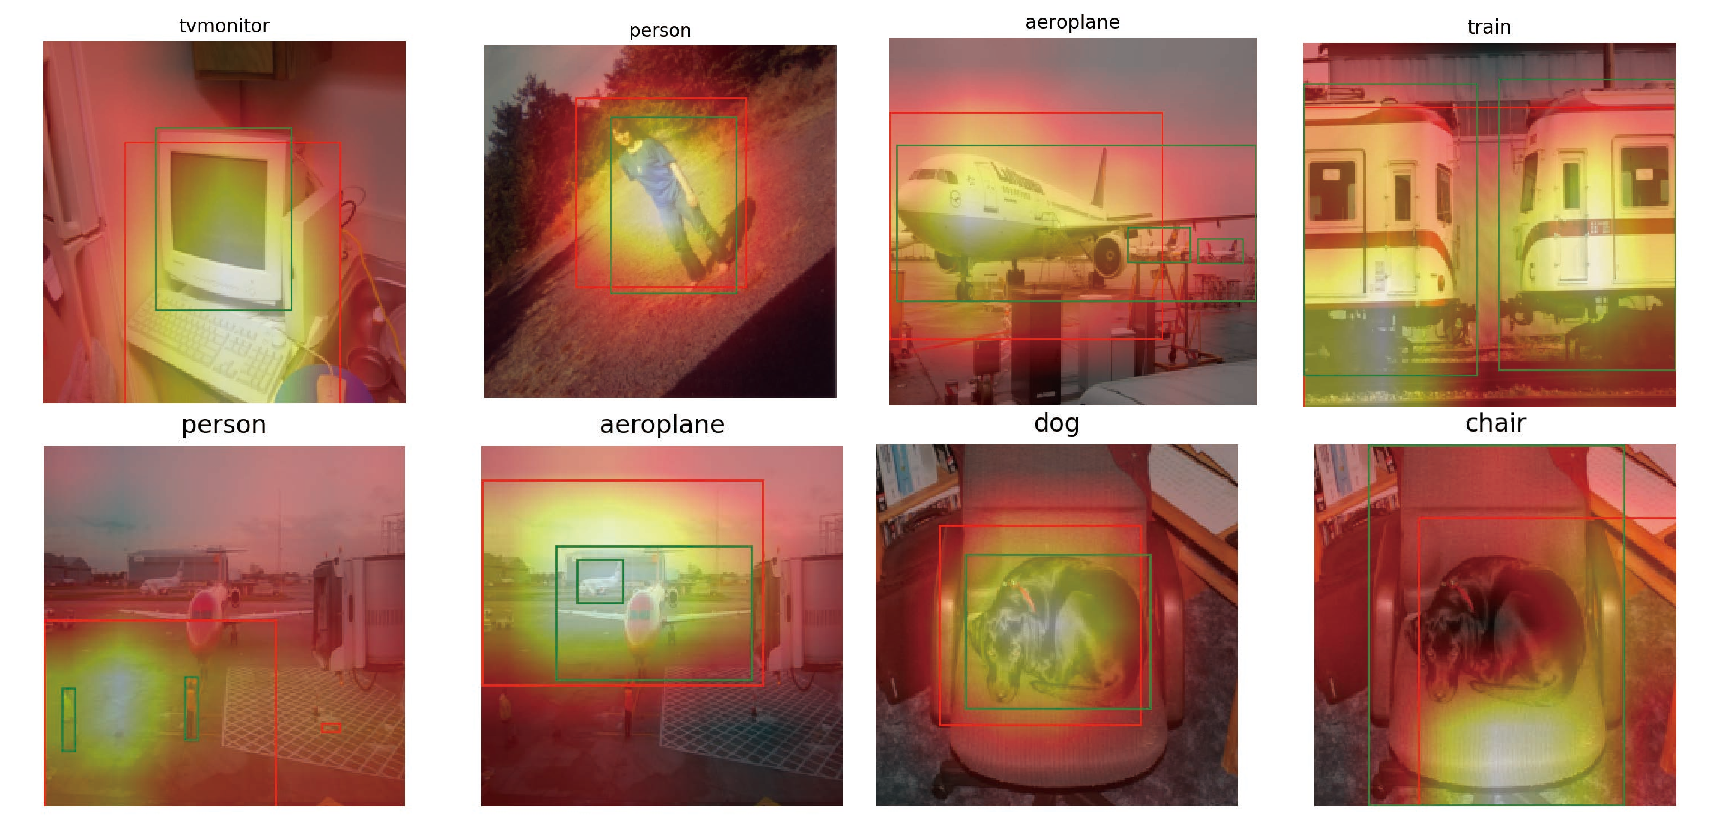
\includegraphics[width=\linewidth]{img/qualitativeLR.pdf}
    \caption{部分结果:原图,CAM ,和 bounding box 的叠加。红色框为检测结果,绿色框为 ground truth}
    \label{fig:qualitative}
\end{figure}

部分结果见图~\ref{fig:qualitative} ,可以观察到,对于图片中有单个明显物体的情况,检测的结果还可以接受。但是对于图片中有多个大小不同的同类物体时,CAM 一般只关注最大的那一个,而且 CAM 一般覆盖范围比较大,得到的 bounding box 一般大小比较大,导致较小物体的检测结果比较差。

此外,将 CAM 视为卷积层的注意力分布的一种表现,我们可以观察到一些有趣的事实,对卷积神经网络的行为模式产生一定的认识。观察~\ref{fig:qualitative} 左上角的图,对应 tv monitor 的 CAM 关注点是电脑和键盘这个整体。事实上,我对测试集的结果进行了进一步的观察,对于 tv monitor 这一类,关注点往往在电脑显示屏和键盘这个整体上,可能是因为,两者往往一起出现,而且都非常有辨识度。

而且,当同类的两种大小相近,位置相近的物体同时出现时,CAM 的注意力会比较平均地分散在两个两个物体中间的位置,这一点可以从右上角的图和左下角的图中看到。

\subsubsection{定量结果}

我们考察了 densenet161/vgg19 w/o Hide and Seek(HaS) 检测结果的 mAP,结果如表~\ref{table:WSOD}。可以看到,DenseNet161 表现要远好于 VGG19,而且采用 HaS 算法训练确实提高了 DenseNet161 的检测 mAP 。但是,加入 HaS 后,两个网络的分类 mAP 都有所降低,这是因为随机掩盖原图像的一些块,确实会提高训练时网络面对问题的难度,而且对于多标签分类问题,这种操作很可能会将一整类的物体全部掩盖,让网络向错误的方向训练,影响准确率。原论文~\cite{singh2017hide}中,处理的都是单标签多分类问题,掩盖原图像的一部分一般不会把整个待分类的物体掩盖住,所以对最终结果的影响不是很大。

\begin{table}[t]
\centering
\caption{WSOD mAP 结果}
\label{table:WSOD}
\begin{tabular}{c|cccc}
\hline
\hline
& \multicolumn{2}{c}{with HaS} & \multicolumn{2}{c}{without HaS}\\
& mAP(WSOD) & mAP(Classification) & mAP(WSOD) & mAP(Classification) \\
\hline
DenseNet161 & \textbf{12.07 \%} & 81.60\% & 11.36 \% & 84.16 \% \\
VGG19 & 5.50 \% & 78.35 \%& 5.98 \% & 79.84 \% \\
\hline
\hline
\end{tabular}
\end{table}

\section{总结}
本次实验中,我们完成了基于深度学习方法的多标签分类和弱监督物体检测任务。我们采用 ML\_GCN~\cite{ML_GCN_CVPR_2019} 方法实现了多标签分类,达到了 0.87 的 mAP ,采用 CAM~\cite{zhou2016learning} 和 Hide and Seek~\cite{singh2017hide} 算法实现了弱监督物体检测,达到了 0.12 的 mAP。

另外,我们实现了一个用于进行深度学习实验的代码框架,具有较好的可扩展性,能够非常方便的进行新算法的实现,训练和测试,所有的工作都是在我们自己的代码框架下复现的。

\section{其他}
\subsection{分工}
\begin{itemize}
    \item 张艺璇:分类任务
    \item 江振宇:检测任务
\end{itemize}

\subsection{进程}
\begin{itemize}
    \item 中期前:搭建框架,用 densenet161 训练 baseline,实现 CAM 的计算
    \item 中期后:实现 ML\_GCN 网络架构,用 CAM 实现弱监督的物体检测,实现 Hide and Seek 等基于 CAM 的提升算法
\end{itemize}

\subsection{代码使用方法}
从 \url{https://cloud.tsinghua.edu.cn/d/5f958eb2797c41a18dd4/} 下载 mAP\_best\_ckp.pth 和  \\WSOD\_besk\_ckp.pth 放在代码的 experiments 下,进入代码根目录(必须是学堂里上传的代码,GitHub 上的代码里没有检测 mAP 的 ground truth 文件),运行

\begin{minted}[linenos, frame=lines]{Python}
python test.py -opt option/test/test_dense161_gcn.json # 多标签分类的测试
python test_WSOD.py -opt option/test/test_dense161_WSOD.json # 弱监督物体检测的测试
\end{minted}

即可进行测试,其他使用方法详见代码的 README.MD

\bibliographystyle{plain}
\bibliography{ref.bib}

\end{document}